\section{Theory}
\label{section: Chapter4/theory}

In Chapter \ref{section: Chapter3}, the mathematical model for single-phase fluid-driven fracture is described ( Section \ref{formulation}). In what follows, this same model is assumed, as all derivations are independent of the system's dimensionality as well as fracture shapes. Since the multi-resolution framework is employed, two coexisting descriptions are used. In a global domain, cracks are assumed to be represented by two-dimensional surfaces embedded in the 3D domain and the governing equations and boundary conditions are those from \eqref{linear momentum balance} - \eqref{pf_ic}, which assume a fixed fracture geometry. In the local domain, the fracture problem is treated with a variational phase-field formulation, given by \eqref{basic u problem}-\eqref{eq:ddot-strong} which assumes flow quantities to be fixed.

A more detailed discussion of the motivation and fundamentals of the multi-resolution method is provided in Section \ref{numerics}. This type of approach is particularly interesting for simulating fluid-driven fracture due to the availability of a discrete fracture at the global level, which simplifies the computation of the fracture apertures that must be coupled to the fluid problem. If a pure phase-field description is used, extracting these apertures becomes a challenging task. In addition to that, a multi-resolution approach can also alleviate the computational cost that comes with the highly-refined grids needed to resolve the fields in a phase-field for fracture formulation. This becomes a remarkable limitation in the context of hydraulic fracturing since the length of fractures is usually on the order of kilometers.

% In a nutshell, it breaks a fracture problem in two separate problems. In the global one, that covers the whole domain, a discrete representation of the fracture is used, but its geometry is assumed to be fixed. To account for crack propagation, a local problem in a vicinity of the fracture front is set up, employing the phase-field method, taking advantage of its flexibility in representing evolving fracture geometries.

An attentive reader will realize that the only part of the multi-resolution algorithm proposed in Chapter \ref{section: Chapter3} that is not extendable to three-dimensions is the propagation step described in  subsection \ref{propagation_step}. In this part of the algorithm, the crack tip location is extracted from the damage field in the local problem and used to inform the global problem as to how to advance the crack. In three-dimensions there is not a single crack tip but instead a fracture front. In addition, while in 2D it is always possible to connect line cuts (which are just line segments) to form an approximation to the crack geometry, in 3D these become planar cuts, which may fail to connect on element boundaries, as shown in Figure \ref{fig:gaps}. Therefore, the way crack propagation is handled needs to be revisited in order to extend the method to three-dimensions.

\begin{figure}[h]
    \centering
    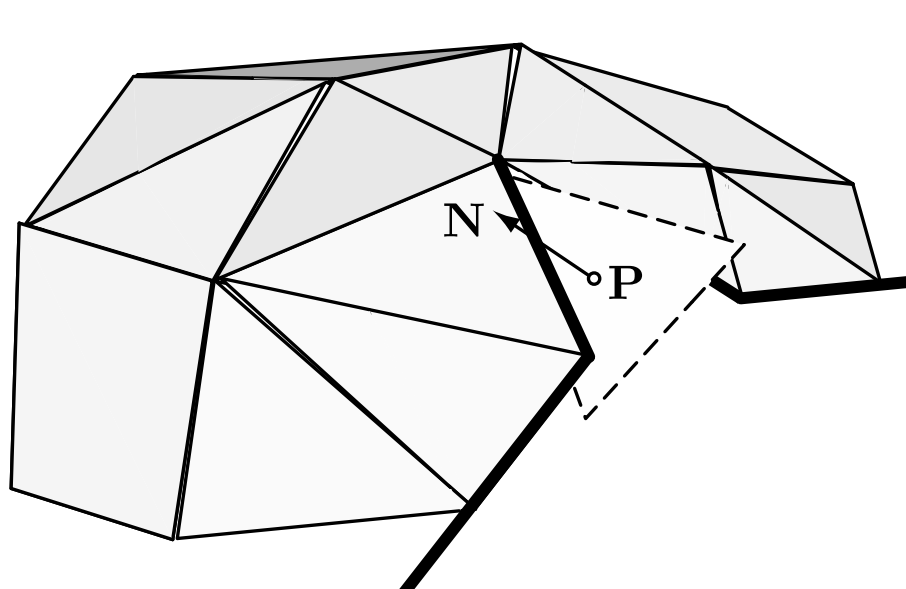
\includegraphics[width=0.6\linewidth]{Chapter4/figures/surface_with_gap.png}
    \caption{Illustrative example of a 3D surface with gaps arising if surface elements do not connect smoothly. Extracted from \cite{gasser20063d}.}
    \label{fig:gaps}
\end{figure}

The first extension discussed in this chapter deals with the case of planar fractures in 3D. The main challenge here consists of tracking the entire fracture front and evolving it according to the damage field computed in the local problem. This is done by defining a discrete set of crack front elements which are investigated for damage throughout the problem execution. The construction of this layer of front elements ahead of the crack is important to preserve the accuracy of the solution, because the absence of a fluid solver in the local problem can lead to spurious unstable solutions\footnote{In hydraulic fracture, the fracture propagation is in general stable because the pressure drops as the fracture volume increases. However, this characteristic only exists when the fluid solver is coupled to fracture propagation.}.  